
\section{Dynamic pipeline}


\begin{figure}[H]
    \centering
    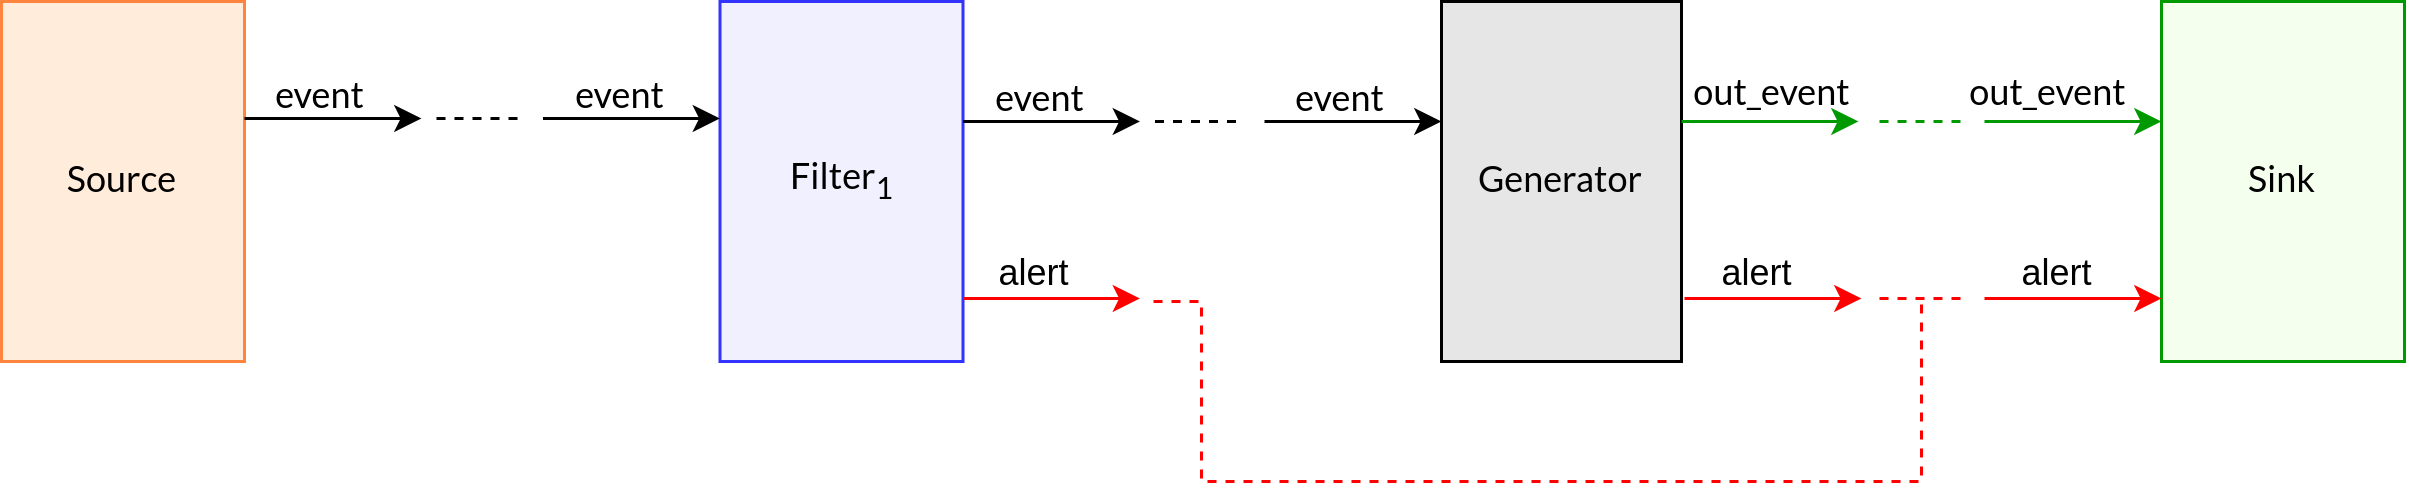
\includegraphics[scale = 0.7]{images/3-Engine/pipeline-schema.png}
    \caption{Pipeline Schema}
    \label{img:pipeline-schema}
\end{figure}

\textcolor{red}{\textbf{TODO: Switch the description, edge and event channel merged in 1 single channel}}\\

Description of the channels:
\begin{itemize}
    \item \texttt{event}: events channel. \textcolor{red}{TODO: Describe the type of events!}
    \item \texttt{alert}: direct channel from the filters (in particular the filter worker) to the sink (it does not go through the Generator, although it has it to be able to give it to the filters so that they are able to write on it)
    \item \texttt{out\_event}: direct dedicated event channel between Generator and Sink.
    \item \texttt{internal\_edge}: edge channel between filter and its worker. Used to communicate to the worker the edges belonging to the filter that the worker needs to process. \textcolor{red}{$\rightarrow$ Now events and not only edges, and also distinguishing between start and end edges on the type of event.}
    \item \texttt{endchan}: synchronization channel between Filter and Worker, to let Filter know whenever Worker is done. To avoid finishing the filter before the worker is actually done. \textcolor{red}{TODO: Include in the drawing}
  \end{itemize}


\begin{figure}[H]
  \centering
  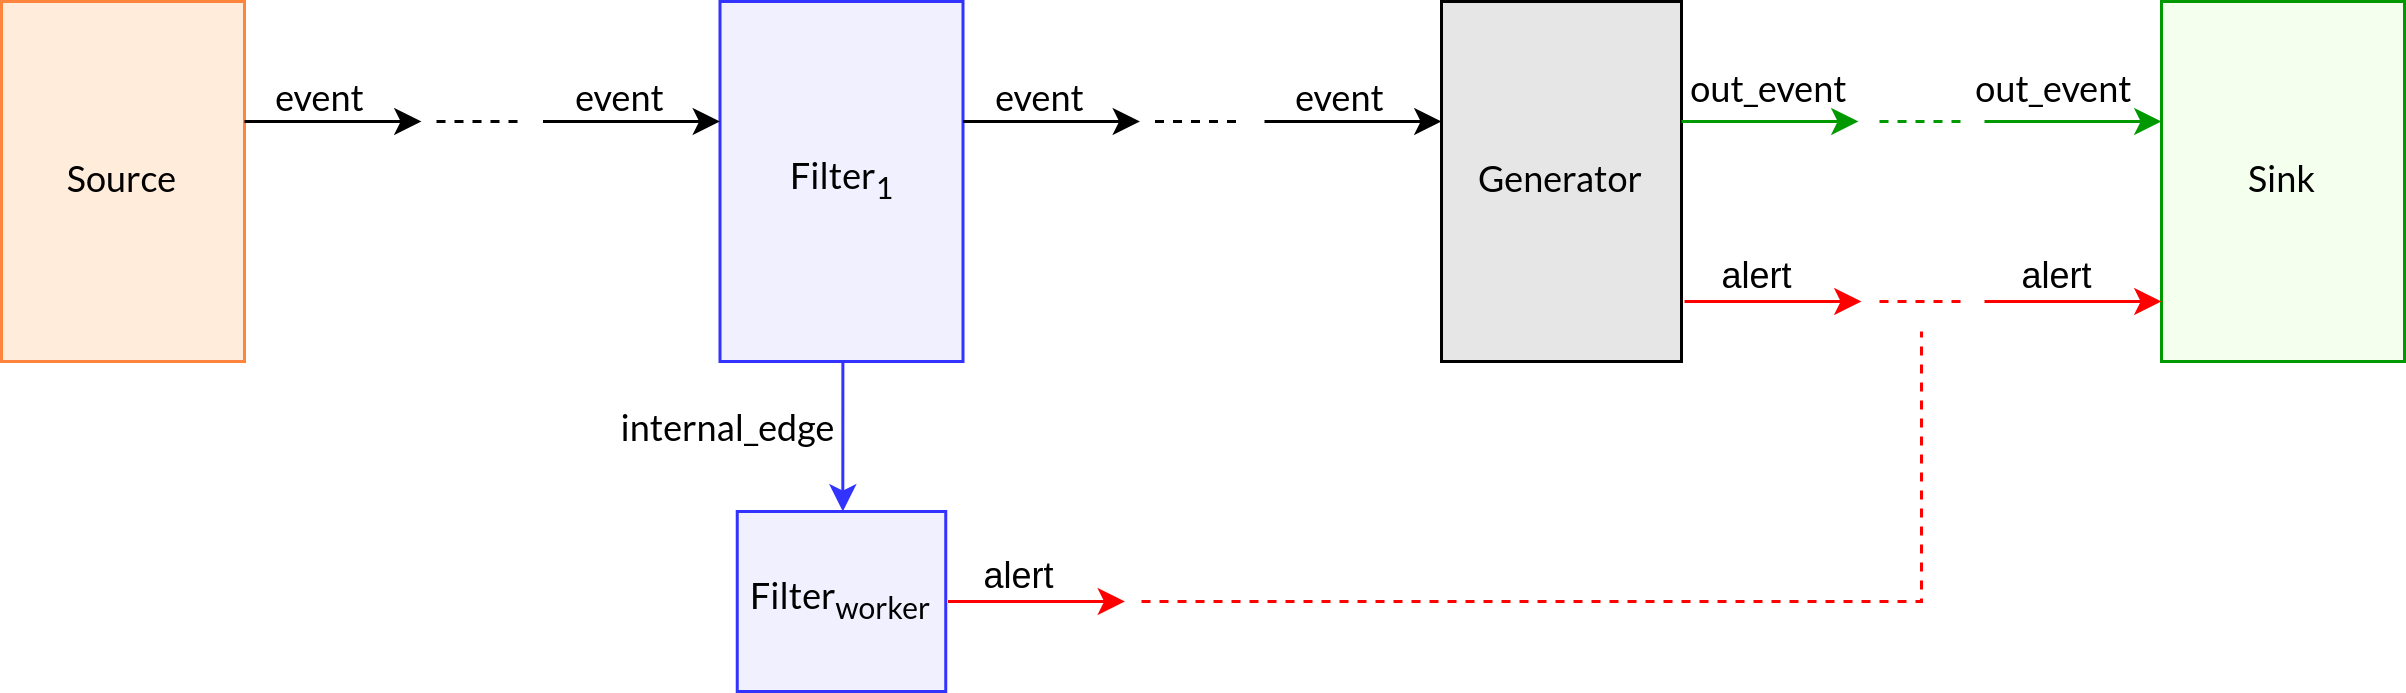
\includegraphics[scale = 0.7]{images/3-Engine/pipeline-schema-filter-detail.png}
  \caption{Pipeline Schema with Filter detail}
  \label{img:pipeline-schema-0}
\end{figure}

\begin{figure}[H]
  \centering
  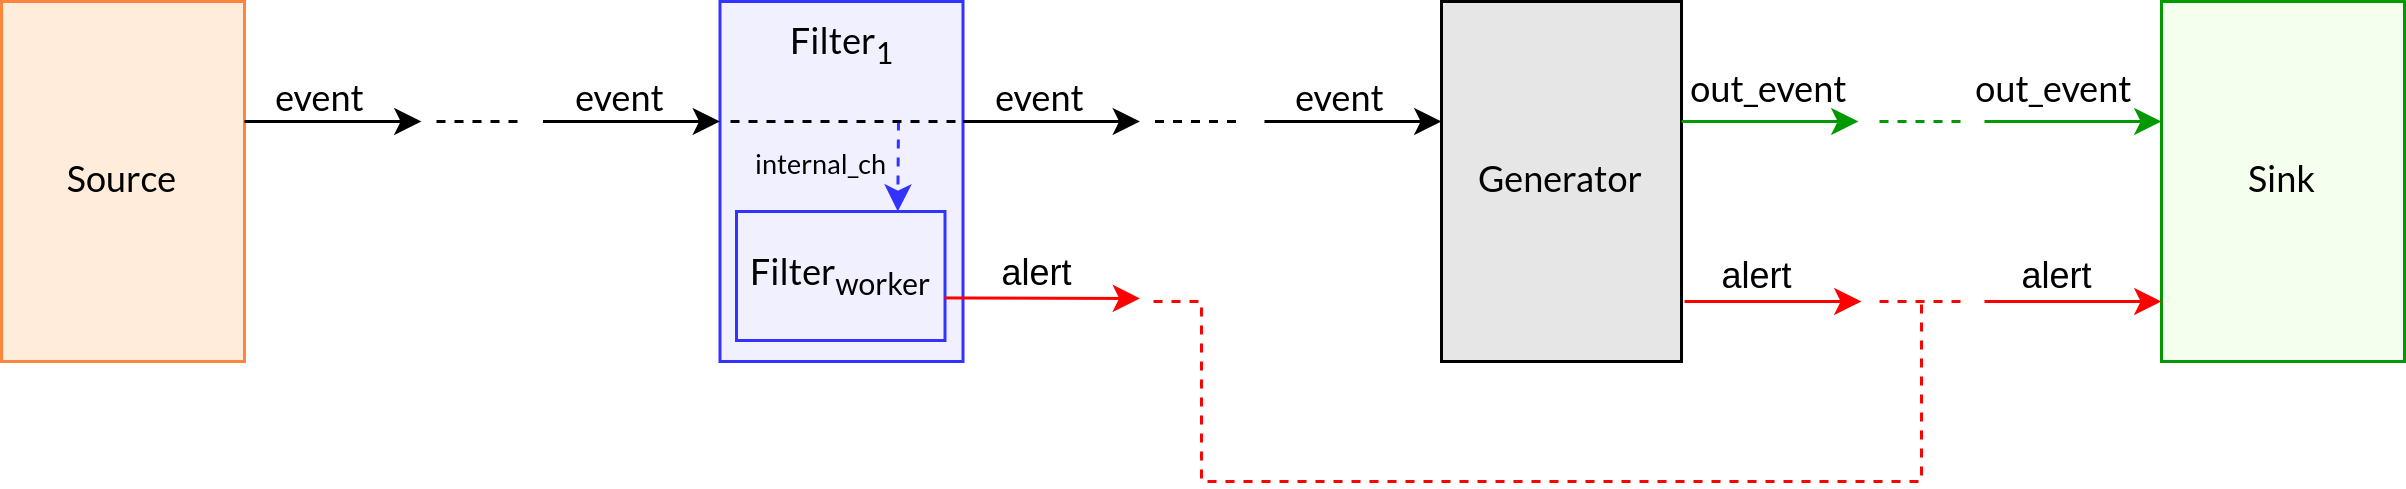
\includegraphics[scale = 0.7]{images/3-Engine/pipeline-schema-filter-detail-1.png}
  \caption{Pipeline Schema with Filter detail 1}
  \label{img:pipeline-schema-1}
\end{figure}


\textcolor{red}{\textbf{Problem detected}\\
If the EOF event is sent through the event channel then it can happen that this event reaches / is treated before the full stream of edges is fully read / processed, leading to
the termination of the processes before the processing of all the edges.\\
Therefore, we decide to merge the edge and the event channel in one single channel!}

Some notes on the implementation decisions:

\subsection{Filter worker}

Options:

\begin{itemize}
  \item External (named) goroutine
  \item \textcolor{green}{$\rightarrow$} Internal anonymous goroutine
\end{itemize}

Advantages of this decision:
\begin{itemize}
  \item Code simplification, the filter worker can access the variables of the scope of the
  filter (no need to pass them as parameters). This is particularly useful in the case of the \texttt{alert} channel, to which the worker is able to write directly. Same in the case of the \texttt{internal\_edge} channel.
\end{itemize}

and in the case of passing the edges of the card from the filter to the filter worker:
\begin{itemize}
  \item Shared buffer using mutex
  \item \textcolor{green}{$\rightarrow$} Channel 
\end{itemize}

In the case of having a shared buffer to communicate the edges between the filter and the worker a mutex is needed. This is because the filter and the worker can possible write and read, respectively, into this buffer at the same time. With it we will avoid race conditions in the sharing of the buffer. However, a channel or other kind of tool would be needed to indicate the worker that there is an edge ready to be read in the buffer. Not having this, would imply to continuosly have the worker requesting the mutex to read from the buffer, even when it is empty and there is no edge to read. 

Therefore as a much more simple alternative, we decided to use an internal channel \texttt{internal\_edge} in between the filter and the worker. With it we avoid having to use a mutex and leading with its derived coordination issues. As a general use case channels are typically used for \emph{passing the ownership of data} which is the case we are dealing with.

Some links:
\begin{itemize}
  \item \href{https://stackoverflow.com/questions/47312029/when-should-you-use-a-mutex-over-a-channel}{When should you use a mutex over a channel?}
  \item \href{https://go.dev/wiki/MutexOrChannel}{Go Wiki - use a mutex or channel?}
\end{itemize}


\begin{figure}[H]
  \centering
  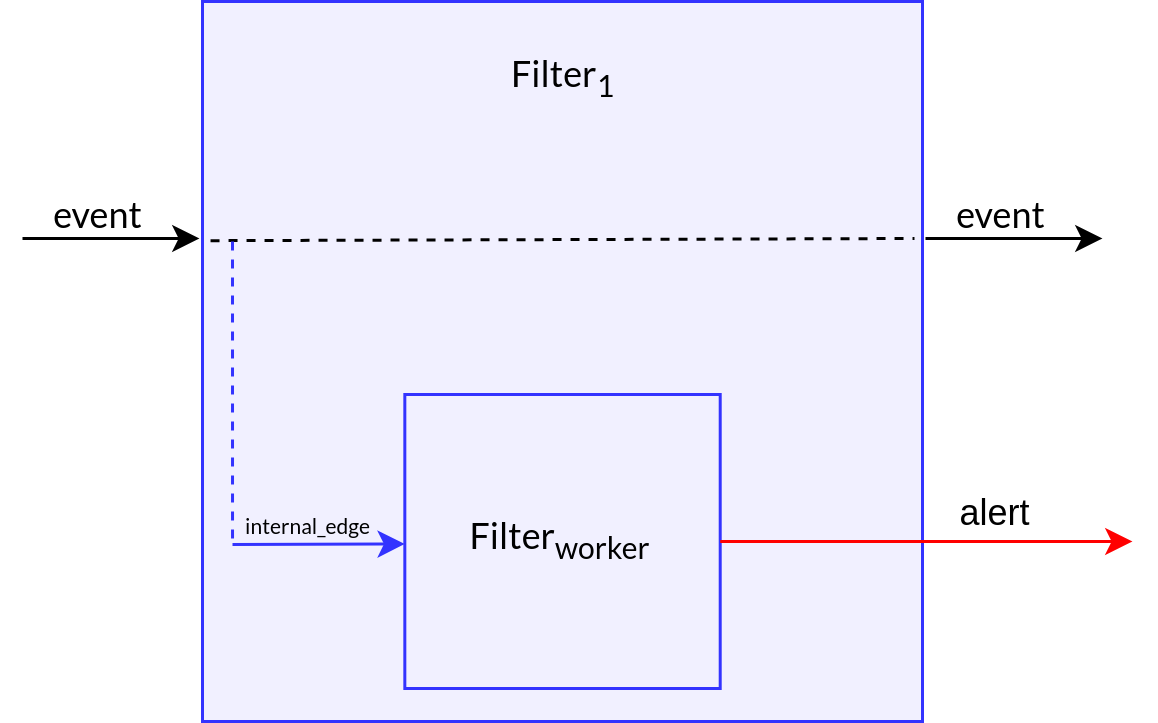
\includegraphics[scale = 0.7]{images/3-Engine/filter-worker.png}
  \caption{Filter Worker detail}
  \label{img:pipeline-schema}
\end{figure}


\section{Multiple cards per filter support}

Use a hash table to index card ids to card subgraphs
\begin{itemize}
  \item key: card id
  \item value: pointer to Graph
\end{itemize}

Note that golang maps are inherently dynamic in size. -> control the desired maximum size by ourselves. 

Management:
\begin{itemize}
  \item Filter
  \begin{itemize}
    \item Reads to check the existance of an entry on the map
    \item Creates the entries on the map (in the corresponding cases)
  \end{itemize}
  \item Worker
  \begin{itemize}
    \item Modifies the entries on the map once they are created
    (Filter does not modify values after the creation of the entry)
  \end{itemize}
\end{itemize}

Conclusion: Safe to do it with a single map and without mutex, since
there can not be concurrent writes on the same map entries. Filter writes
on the creation and then it is only the worker who writes on that entry after
the creation of the entry by the filter.

\textcolor{red}{Issue: "fatal error: concurrent map read and map write"}

More details -- in Golang it is not defined what happens when we have simultaneous read/write operations:

\begin{itemize}
  \item \href{https://go.dev/doc/faq#atomic_maps}{Maps Atomicity}
  \item \href{https://go.dev/doc/go1.6}{Runtime. Use of maps}
  \item \href{https://go.dev/blog/maps}{Golang maps. Concurrency}
  \item \href{https://groups.google.com/g/golang-nuts/c/_XHqFejikBg?pli=1}{Golang maps concurrency - blog}
\end{itemize}

\subsection{Solution}

2 hash tables (to avoid race conditions in concurrent access by filter \& worker):
\begin{itemize}
  \item \texttt{cardList}: to control the belonging cards to the filter. Only access by filter.
  \item \texttt{cardSubgraph}: to map each belonging card to its corresponding subgraph. Only access by worker.
\end{itemize}

Note that, all the edges that we pass to the worker are of cards that belong to the corresponding filter. This means that we do not need to do any check on the \texttt{cardSubgraph} map.

\textcolor{red}{\rule{\linewidth}{0.5mm}}
\textcolor{red}{TODO: Pendiente de explicar -- revisar "dynamicPipeline.tex}

\begin{itemize}
    \item Algorithms of filter, filterWorker, and the rest of stages.
    \item Completion of tx when arriving closing interaction edge.
    \item Data structure description of volatile subgraph.
    \item Description that anomalous tx are also stored in the subgraph.
\end{itemize}


% TODO: Explicar el dynamic pipeline y su relación / uso con la detección de patrones de fraude:
% filtros y construcción de subgrafos voltátiles en ellos, + un stable graph compartido entre todos como una especie 
% de database del banco

\textcolor{red}{\rule{\linewidth}{0.5mm}}
\textcolor{red}{TODO: Reformulate this description -- single window VS windowed approach}
\begin{graysection}
\subsubsection{Structure description}

% TODO:
% - Describir la estructura de los filters: channels y como se relacionan, flujo, creación,
% eliminación de un filtro, reconexión... EN GENERAL! SIN ESPECIFICAR PARA TX/ATMS
% -> mirar referencias (de otros TFGs/TFMs, artículos de Edelmira...)
% - Explicar lo del filter-worker y por qué se tiene. Básicamente para evitar que se interrumpa el flujo de transacciones en caso de que un filtro tarde en procesar o realizar alguna operacion con alguna transaccion que pertenece a él. El procesamiento se hace en el filter worker y mientras el filter por encima actua como una especie de filtro/ tajadera que desvía las transacciones del filtro al worker y las que no las deja seguir fluyendo por el canal de transacciones hacia los filtros posteriores sin interrumpir el flujo de esta manera.

% NOTE: Esto podría ser modificado y tener más de 1 card por filtro
In principle, we are going to dedicate one filter per card. A filter will be tracking the activity of a card during a certain active time period, by filtering all the transactions belonging to that card and keeping a \textit{windowed} volatile subgraph that contains the transactions of the filter associated card during the last fixed window of time. Once a certain time period has passed without registering any activity on the filter, that is, there are no transactions associated with the card it \textit{hosts}, the filter will be destroyed and the pipeline reconnected accordingly. 
Note that the deletion of the filters after a certain time of inactivity is done due to the huge overhead that it would imply to keep them all simultaneously whenever we are considering a big amount of cards.

\subsubsection{Transaction flux}

\subsubsection{Filter's management and volatile subgraph}

% 0. Qué es. Para qué lo necesito. 
% 1. Cómo es. Data structure description selection
% 2. Cómo funciona. Requisitos funcionales. Descripción funcionamiento.
% * Comentar data structure y operaciones relacionadas: newGraph, update, addAtEnd
% * Tiempo de vida filtro, gestión de esto, eliminación del filtro...

% 0. Qué es. Para qué lo necesito. 
With the purpose of tracking the activity of each of the cards on each of the filters we build a \textit{windowed} volatile subgraph, which has as edges all the transactions belonging to the card that were registered during the last fixed window of time. This volatile subgraph is going to be updated based on the flux of transactions of the pipeline. We need to have this volatile continuously updating subgraph per each of the cards as a \textit{short-term memory} register of the last transactions of a card during a certain window of time, so that whenever a new transaction comes we can make associations/relations with the transactions registered on that last window of time and possibly alert of a potential fraud whenever it is the case.\\
Therefore, the continuous update consists of adding new incoming transactions and discarding the old transactions that fall outside the fixed window of time. This ensures that only transactions inside the fixed window of time are considered to do associations for fraud detection. 
% 1. Cómo es. Data structure description selection
Based on these premises, the data structure to keep the volatile subgraph needs to have two main properties:
\begin{itemize}
    \item Efficient to add new transactions/edges.
    \item Efficient to delete the transactions/edges that are outdated in relation to the fixed \textit{window} of time.
\end{itemize}

Considering that the transactions arrive ordered in time, a linked list was selected as a suitable approach to save the transactions/edges ordered by timestamp. It allows a cheap and easy way to manage the volatile subgraph by adding the new transactions at the tail of the list and deleting the outdated ones from the head of the list. The golang \href{https://pkg.go.dev/container/list}{\texttt{container/list}}, implemented as a doubly linked list was used as an already given implementation of the desired linked list.

\textcolor{cyan}{Another possible alternative considered was the golang \texttt{[] slice} which is a dynamically-sized array. The problem of it was the inefficiency on the deletion from the head of the slice, which had a time complexity of 
$O(n)$, where $n$ is the number of elements in the slice, since it required shifting all the remaining elements to the left.}

Another aspect to consider is the deletion of the filter whenever no transactions related to it are registered after a long period of time. Note that the deletion of the filters after a certain time of inactivity is done due to the huge overhead that it would imply to keep them all simultaneously whenever we are considering a big amount of cards.

The filter's data structure and the operations related to it are described in what follows.

% 2. Cómo funciona. Requisitos funcionales. Descripción funcionamiento.
% * Comentar data structure y operaciones relacionadas: newGraph, update, addAtEnd
% * Tiempo de vida filtro, gestión de esto, eliminación del filtro...
\paragraph{Data Structure}

\begin{center}
\lstset{style=golangStyle}
\begin{lstlisting}[caption={filter subgraph data structure}]
type Graph struct {
	last_timestamp time.Time
	edges          *list.List
}
\end{lstlisting}
\end{center}

The filter inner data structure \texttt{Graph} contains the linked list needed to save the volatile subgraph: \texttt{edges}, which is a linked list of transactions (\texttt{Edge}) belonging to the filter within the fixed window of time (see an example in Figure \ref{img:pipeline-subgraph}), and a timestamp: \texttt{last\_timestamp} which saves the timestamp of the last edge that was added to the filter's subgraph. This is used to check for the deletion of the filter in the case of a long time of \textit{inactivity}.

\begin{center}
\lstset{style=golangStyle}
\begin{lstlisting}[caption={Edge of the volatile subgraph, a transaction belonging to the filter}]
// It is an edge of the volatile subgraph
type Edge struct {
	Number_id string    // Card id
	ATM_id    string    // ATM id
	Tx_id     int64     // transaction id
	Tx_start  time.Time // transaction start date time (DD/MM/YYYY HH:MM:SS)
	Tx_end    time.Time // transaction end date time (DD/MM/YYYY HH:MM:SS)
	Tx_amount float32   // transaction amount
}
\end{lstlisting}
\end{center}

\begin{figure}[H]
    \centering
    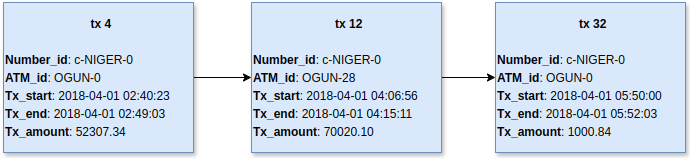
\includegraphics[scale = 0.45]{images/Pipeline/subgraph.png}
    \caption{Subgraph \texttt{edges} linked list of transactions of the \texttt{c-NIGER-0} card filter example}
    \label{img:pipeline-subgraph}
\end{figure}

\paragraph{Operations}
The operations related with the inner filter data structure are the following:

\begin{itemize}
    \item \texttt{NewGraph()}: Creates a new \texttt{Graph} data structure. This is done on the creation of the filter.
    
    \item \texttt{AddAtEnd(e Edge)}: Adds a new edge. Appends a new edge at the end of the list \texttt{edges} and updates the \texttt{last\_timestamp} variable with the \texttt{Tx\_end} time of the new added edge. This operation is done whenever a new transaction edge of the associated card arrives to the filter.
    
    \item \texttt{Update(timestamp time.Time)}: Given a certain datetime, it updates the subgraph, starting from the first edge of the \texttt{edges} list, by eliminating those that are outdated with respect to this datetime. An edge $e$ is outdated  whenever its time difference with respect to the incoming timestamp is greater than the fixed window time constant \texttt{timeTxThreshold}. That is, whenever: $$timestamp - e.Tx\_end \geq timeTxThreshold$$
    This operation is done in two situations:
    \begin{itemize}
        \item $edge \in filter$ ($filter.Number\_id = edge.Number\_id$) Whenever the transaction edge belongs to our filter. Before performing the \texttt{AddAtEnd} operation we perform the \texttt{Update} operation with the timestamp of the new transaction. This ensures that only transactions inside the fixed window of time are considered to do associations for fraud detection. 
        \item $edge \notin filter$ ($filter.Number\_id\ \neq edge.Number\_id$) Whenever a transaction edge passes through our filter but it does not belong to it. We take its timestamp as the \texttt{timestamp} parameter of the \texttt{Update} operation.
    \end{itemize}
    
    \item \texttt{CheckFilterTimeout(timestamp time.Time) bool}: Given a timestamp, it tests if the filter has to be deleted due to a long time of detected \textit{inactivity}. A filter is decided to be deleted if the time difference between the last edge of the subgraph (saved in the \texttt{last\_timestamp} variable) and the incoming \texttt{timestamp} is greater than the fixed \texttt{timeFilterThreshold} time constant: $$timestamp - last\_timestamp \geq timeFilterThreshold$$
    This operation is only performed whenever $edge \notin filter$, taking its timestamp as our parameter, in particular before the \texttt{Update} operation, since in the case the filter needs to be deleted, the \texttt{Update} operation will no longer have to be performed.

    \item \texttt{CheckFraud(new\_e Edge) bool}: \textcolor{blue}{TODO: This is the temporal approximate approach} So far, it is assumed that the current volatile subgraph of the filter is correct (in the sense that it is considered to be free of anomalous transactions). For the moment, only the kind of fraud explained at section \ref{fraud-pattern-1} is checked. \textcolor{blue}{More specifically, the way to perform the check is ONLY between the new incoming edge belonging to the filter \texttt{new\_e} and the last edge that was added to the volatile subgraph. And if, this kind of fraud pattern is matched then an alert is output and this last edge is considered to be anomalous and therefore it is not added to the volatile subgraph of the filter}. 
    
\end{itemize}

With these operations, a summary of the algorithmic behavior of a filter can be seen in the flow diagram on Figure \ref{diag:filter-flow}.

% TODO: Poner ejemplos con dibujitos
% TODO: Diagrama de flujo / casos, para aclarar bien los diferentes casos y qué hago en cada situación
\begin{figure}[H]
    \centering
    \begin{tikzpicture}[node distance=2cm]
\node (start) [startstop] {New Filter (Edge e)};
\node (creation) [process, below of=start] {
    \texttt{NewGraph()}\\
    \texttt{AddAtEnd(e)}
};
\node (while) [process, below of=creation]{in: new edge};
\node (edgeInFilter) [decision, below of=while, yshift=-1cm] {$edge \in filter$};

\node (edgeFilterYes) [process, right of=edgeInFilter, xshift=3cm, text width=4cm] {
    \texttt{Update(edge.Tx\_start)}
    \texttt{AddAtEnd(edge)}
    \texttt{CheckFraud()}
};
\node (filterTimeout) [decision, below of=edgeInFilter, yshift=-2.5cm, text width=3.1cm] {\texttt{CheckFilterTimeout\\(edge.Tx\_start)}};
\node (filterTimeoutNo) [process, right of=filterTimeout, xshift=7cm, text width=4cm] {
    \texttt{Update(edge.Tx\_start)}
};
\node (stop) [startstop, below of=filterTimeout, yshift=-2cm] {Stop};

\draw [arrow] (start) --  (creation);
\draw [arrow] (creation) -- (while);
\draw [arrow] (while) -- node[anchor=east] {edge} (edgeInFilter);
\draw [arrow] (edgeFilterYes) |- (while);
\draw [arrow] (edgeInFilter) -- node[anchor=south] {yes} (edgeFilterYes);
\draw [arrow] (edgeInFilter) -- node[anchor=east] {no} (filterTimeout);
\draw [arrow] (filterTimeout) -- node[anchor=south] {no} (filterTimeoutNo);
\draw [arrow] (filterTimeoutNo) |- (while);
\draw [arrow] (filterTimeout) -- node[anchor=east] {yes} (stop);
\end{tikzpicture}

    \caption{Filter flow diagram}
    \label{diag:filter-flow}
\end{figure}

\paragraph{Considerations}
\begin{itemize}
    \item So far, the way to perform the \texttt{Update} and the \texttt{CheckFilterTimeout} operations could be described as a kind of \textit{filter lazy updating}, since only the filters located before the filter to which the transaction edge finally belongs are updated with the timestamp of that edge. Whereas the filters located after this filter will not be updated with this timestamp. The cause of this is that once the edge is filtered to its corresponding filter, it \textit{sinks} into it, and therefore it is not propagated to the consecutive filters. See the case on Figure \ref{img:pipeline-update-issue}, where if a transaction edge was to belong to the filter F3, then only the filters F1, F2 and F3 will be updated accordingly to the timestamp of this edge, whereas the filter F4 will not be updated in this case.
    \begin{figure}[H]
        \centering
        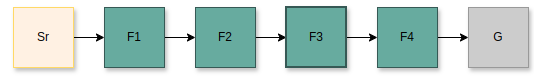
\includegraphics[scale = 0.45]{images/Pipeline/update-issue.png}
        \caption{Pipeline \textit{filter lazy updating} example}
        \label{img:pipeline-update-issue}
    \end{figure}
    However, this is not necessarily a problem. The reason is that the filter will perform these operations later in the future. Note that in the case that the edge belongs to the filter, the \texttt{Update} operation will be performed just before doing the \texttt{AddAtEnd} operation as it was already mentioned in the description of the \texttt{Update} operation. \textcolor{red}{Note that to avoid this "problem" another approach could be done like doing a timestamp channel or passing all the edges until the end of the pipeline.} 
    \item Due to the nature of the management of the filter's lifetime and subgraph updating, it can be the case that our filter subgraph is empty, although the filter is still alive. We can arrive to this situation by having deleted all the edges of the filter subgraph since they were outdated, but still the \texttt{timeFilterThreshold} time has not yet passed. However, thanks to the saved \texttt{last\_timestamp} variable we do not need to save the last edge or do anything but comparing the incoming timestamp with this 
    \texttt{last\_timestamp} variable (calling the function \texttt{CheckFilterTimeout()}).
\end{itemize}
% - last_timestamp parameter helps avoid having to save the last edge completely. The case of the subgraph being empty % but the filter still be active case

% TODO: Tests!!!!
% 1. AddAtEnd -> no añadir...
% 2. Update   -> añadir?
% 3. Filter timeout  -> añadir? (*) igual sólo añadir este, pues es más completo e incluye a los anteriores
\end{graysection}